\documentclass[compress]{beamer}

\setlength{\unitlength}{\paperwidth}

\usepackage{graphicx, subfigure}
\usepackage{multimedia}
\usepackage{hyperref}
%\usepackage{verbatim}
\usepackage{listings}
\usepackage{caption} % For linebreaks in captions

\newcommand{\mb}[1]{\mathbf{#1}}

\mode<presentation>
{
  \useoutertheme{split}
  \setbeamercolor{separation line}{use=structure,bg=structure.fg!50!bg}
  \usefonttheme{structurebold}
  
  \setbeamertemplate{navigation symbols}{}
  % or ...

  % \setbeamercovered{transparent}
  % or whatever (possibly just delete it)
}


%%\usepackage[danish]{babel}
%%\usepackage[utf-8]{inputenc}
\usepackage{times}
\usepackage[T1]{fontenc}


\title[RcppAD]
{A comparison between ADMB \& RcppAD}

\author[K. Kristensen, A. Nielsen, C.W. Berg ]% [Author, Another] % (optional, use only with lots of authors)
{Kasper Kristensen, Anders Nielsen, Casper W. Berg}

\date[September 2013] % (optional, should be abbreviation of conference name)
{September, 2013}

\begin{document}

\begin{frame}[plain]
  \titlepage
\end{frame}

\begin{frame}
\frametitle{RcppAD Intro}

\begin{itemize}
  \item ADMB inspired R-package
  \item Combines external libraries: cppAD, Eigen, CHOLMOD
  \item Continuously developed since YYYY, $\sim 1000$ lines of code
  \item Implements Laplace approximation for random effects
  \item C++ Template based
  \item Automatic sparseness detection
  \item Parallelism through BLAS
  \item Parallel user templates
\end{itemize}


\end{frame}

\begin{frame}
  \frametitle{Example 1: Linear regression}
\end{frame}


\begin{frame}
  \frametitle{Example 2: Multivariate random walk}
\begin{columns}
    \begin{column}{0.5\textwidth}
      \begin{align*}
        \mb{X}_{t+1} &= \mb{X}_t + \mb{\varepsilon_t} \quad , \mb{\varepsilon_t} \sim N(\mb{0},\Sigma) \\
        \mb{Y}_t &= \mb{X}_t + \mb{\eta_t} \quad , \mb{\eta_t} \sim N(\mb{0},\mb{\sigma}_Y^2 \mb{I}) \\
           \Sigma_{i,j} & = \rho^{|i-j|}\sigma_{i}\sigma_{j}  
      \end{align*} 
     States (random effects) $\mb{X}$, Observations $\mb{Y}$.  
     Parameters: $\mb{\sigma}, \mb{\sigma_Y}, \rho$.
      
    \end{column}
    
    \begin{column}{0.5\textwidth} 
    \begin{figure}[!htb]
      \centering
      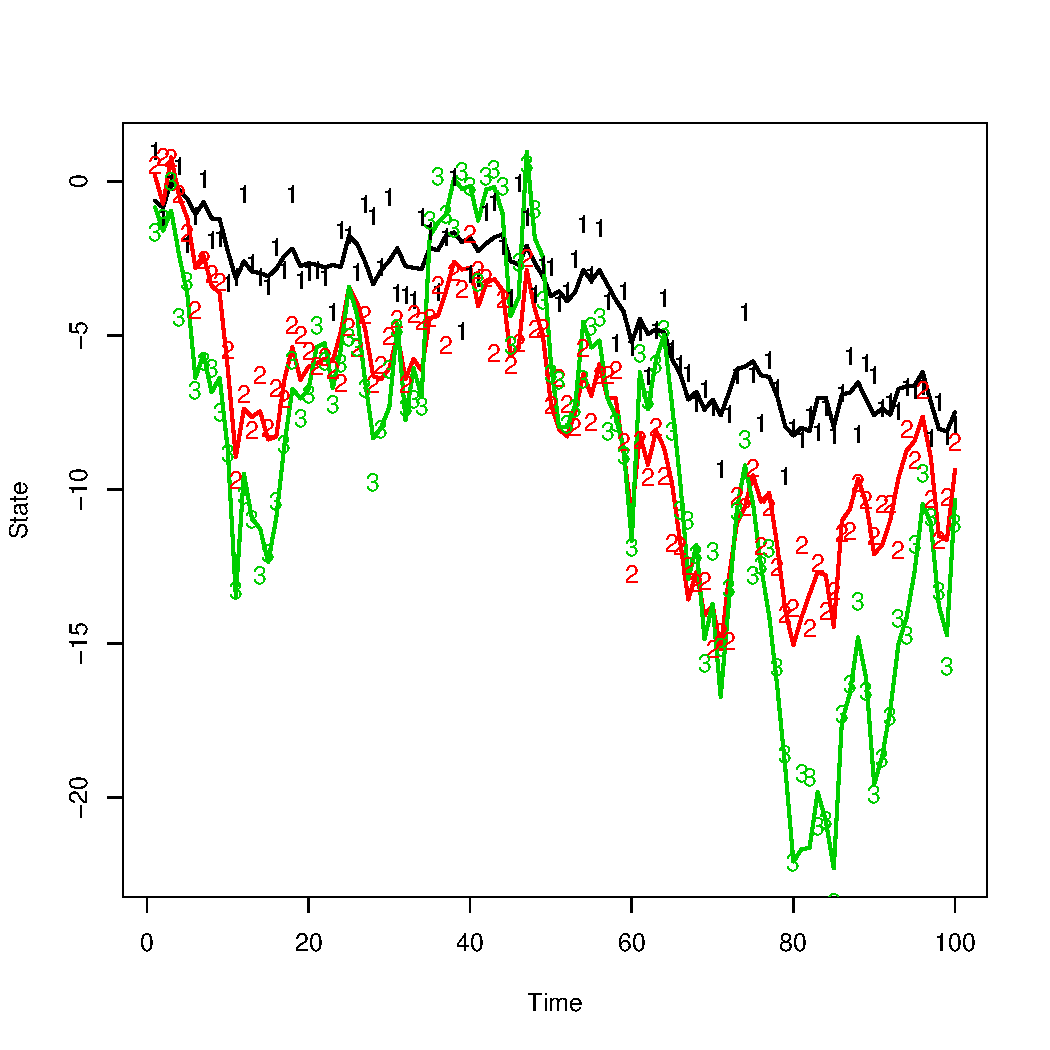
\includegraphics[width=1.0\textwidth]{results/rwplot.pdf}
    \end{figure}

  \end{column}
\end{columns}
\end{frame}

{
\usebackgroundtemplate{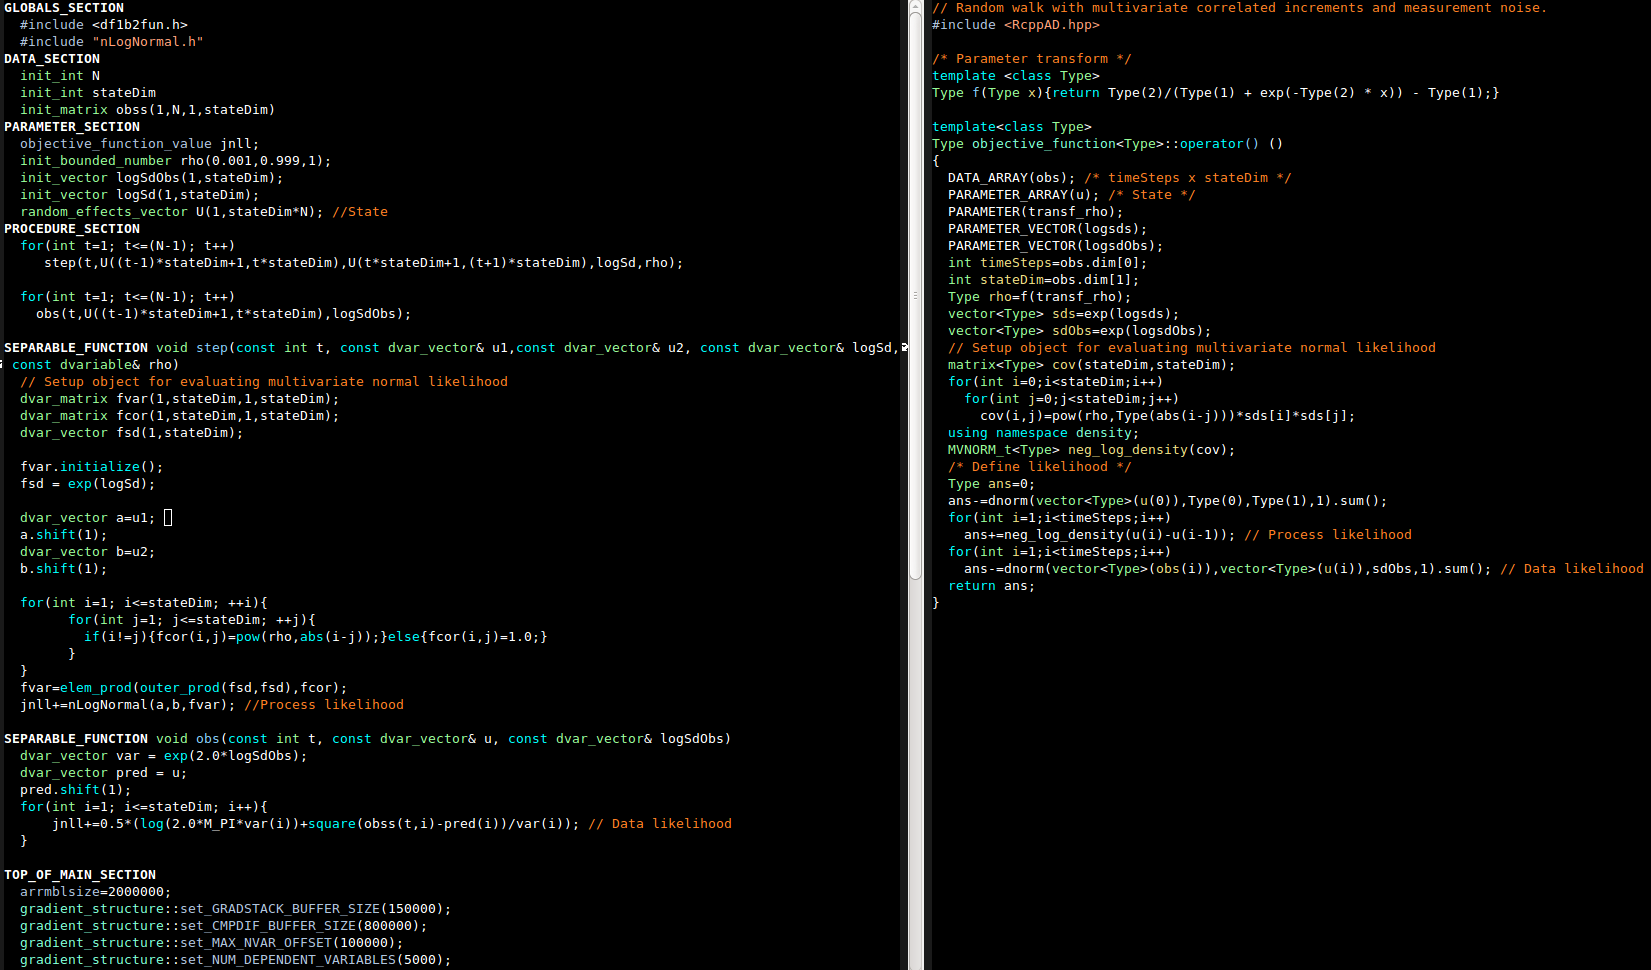
\includegraphics[width=\paperwidth,height=\paperheight]{results/rw.png}}
\begin{frame}[plain]
\end{frame}
}

\begin{frame}
  \frametitle{Example 2: Results (timings)}
  \begin{columns}
    \begin{column}{0.5\textwidth}
      \small{
      % latex table generated in R 3.0.1 by xtable 1.7-1 package
% Mon Sep 16 14:56:17 2013
\begin{table}[ht]
\centering
\begin{tabular}{cccc}
  \hline
 & 3 & 5 & 7 \\ 
  \hline
ADMB & 22.74 & 55.93 & 144.47 \\ 
  TMB & 0.91 & 1.63 & 3.85 \\ 
  Speed-up & 24.88 & 34.34 & 37.56 \\ 
   \hline
\end{tabular}
\caption{Runtime in seconds for multivariate random walk example.} 
\end{table}

      }
    \end{column}
    
    \begin{column}{0.5\textwidth} 
    \begin{figure}[!htb]
      \centering
      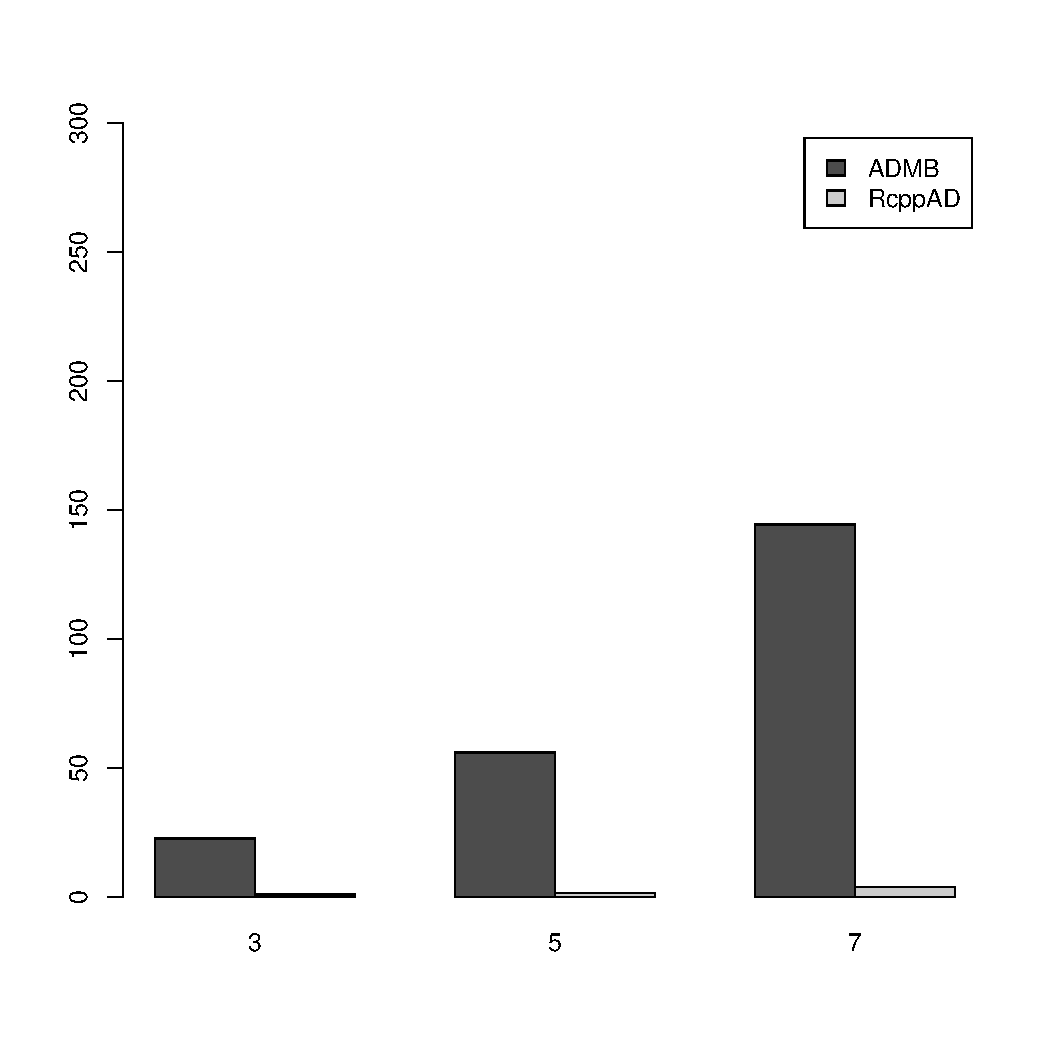
\includegraphics[width=1.0\textwidth]{results/timings.pdf}
    \end{figure}

  \end{column}
\end{columns}
 
\end{frame}

\begin{frame}
  \frametitle{Parallel user templates intro}
\end{frame}

\begin{frame}
  \frametitle{Parallel Code}
\end{frame}

\begin{frame}
  \frametitle{Results: benchmark plot}
\end{frame}


\begin{frame}
  \frametitle{Parallel Code with multicore package}
\end{frame}


\begin{frame}
  \begin{itemize}
    \item[-] Slow compile times
    \item[-] Standalone applications not possible
    \item[-] Fewer built-in specialized functionalities (e.g. profile-likelihood, \texttt{sd\_report\_number} etc.)
    \item[-] Sparse documentation
    \item[-] Depends on external libraries
  \end{itemize}
\end{frame}

\begin{frame}
  \begin{itemize}
    \item[+] Fast run times
    \item[+] The use of external libraries means a compact code base that is highly optimized
    \item[+] Can handle very high dimensional problems ($\sim 10^6$ random effects)
    \item[+] No \texttt{SEPARABLE\_FUNCTION} construct needed, fully automatic sparseness detection
    \item[+] Full R integration -- no need for data+results import/export
    \item[+] No use of temporary files on the disc
    \item[+] Template based -- no code duplication needed as for \texttt{df1b2variable}s etc.
    \item[+] Analytical Hessian for fixed effects.
    \item[+] High-level parallelization with \texttt{multicore} package. 
  \end{itemize}
\end{frame}


\end{document}